\section{Zyklische Belastung}
    \subsection{Ermüdung:}
        Progressive Shädigiung durch zyklische Belastung $\rightarrow$ Riss $\rightarrow$ Dauerbruch\\
        Einflüsse: 3D Spannungszustand, Temp., Korr., Zeit, Frequenz d Zyklen, Kerbwirkung, Mittelspannung, Eigenspannungen, Kumulative Ermüdung, Oberfläche
        \subsubsection{Allgemeines Vorgehen}
            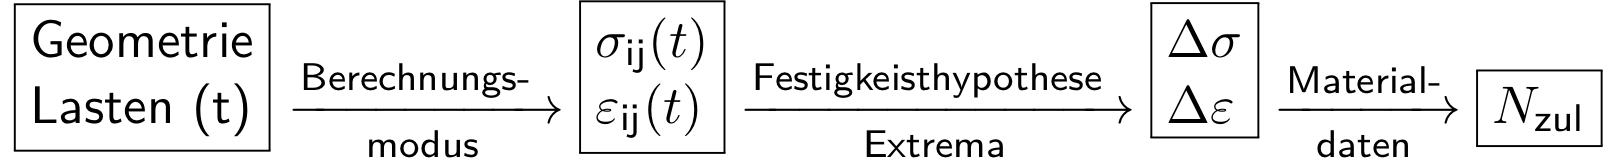
\includegraphics[width=\linewidth]{06/allg_vorgehen.jpeg}
        \subsection{Dauer- \& Zeitfestigkeit:}
            \begin{minipage}{\linewidth}
                \begin{itemize}
                    \item bis $10^3-10^4$ Zyklen: LCF (low cycle fatigue - Kurzzeitfestigkeit)
                    \item $10^3-10^4$ bis $10^6$: HCF (high cycle fatigue - Langzeitfestigkeit)
                    \item ab $10^6-10^7$: Dauerfestigkeit - $\sigma_W$: Wechselfestigkeit
                \end{itemize}
            \end{minipage}
    \subsection{Einfluss der Mittelspannung aud Dauerfestigkeit:}
        \[\sigma_m=\frac{\sigma_u+\sigma_o}{2}; \quad R=\frac{\sigma_u}{\sigma_o} \quad \sigma_m \uparrow, R \uparrow (\sigma_o >0) \rightarrow N_{zul} \downarrow\]
        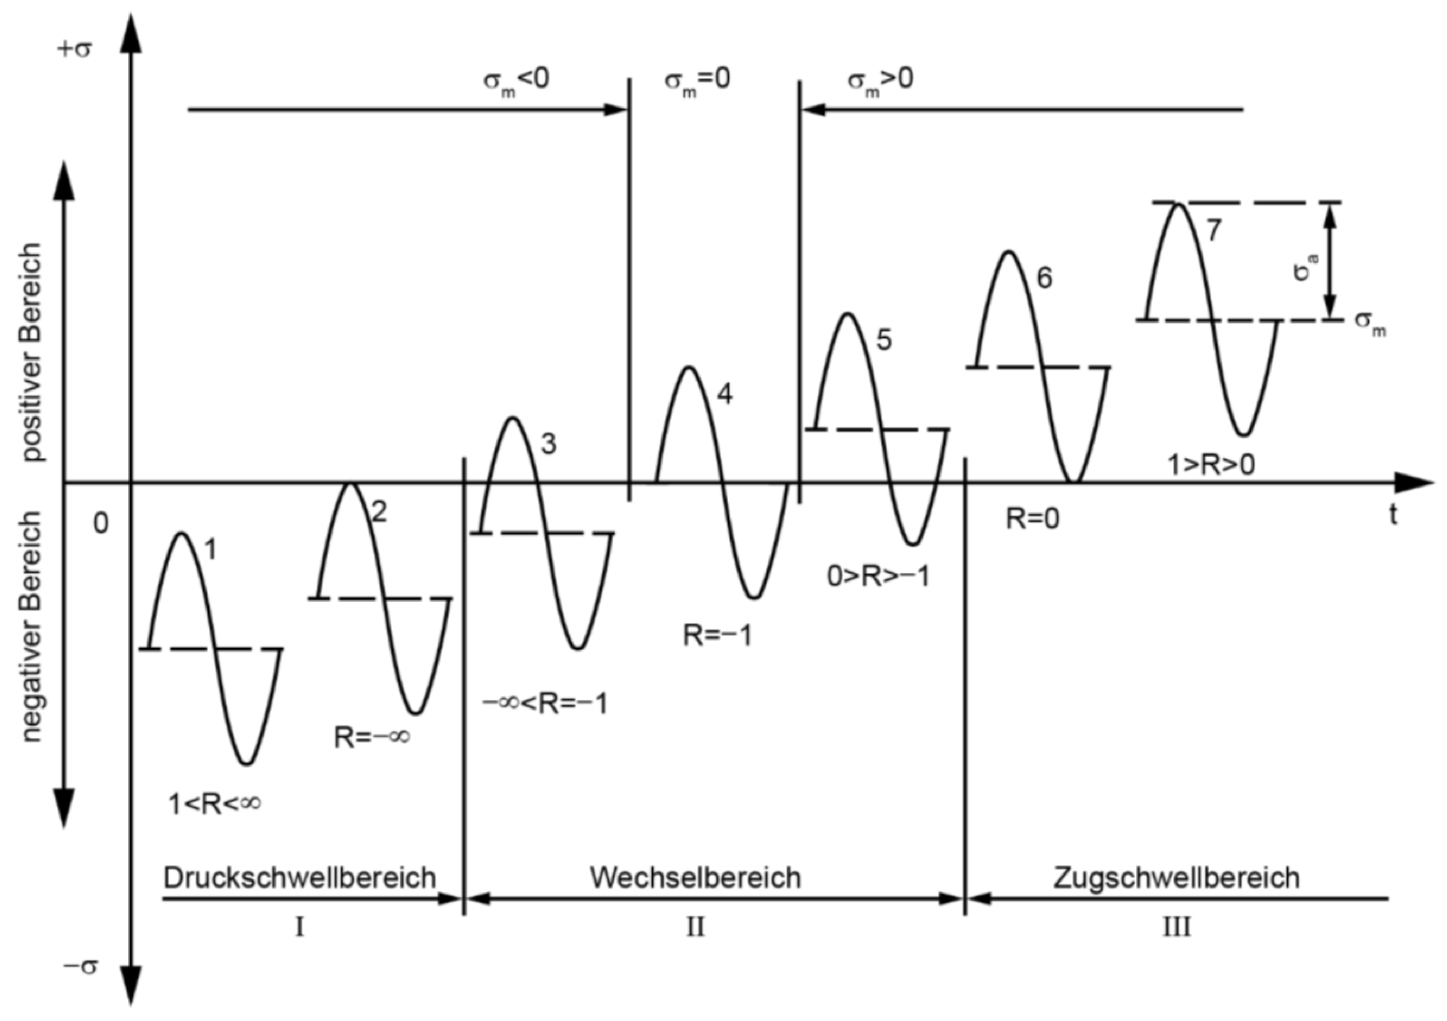
\includegraphics[width=0.6\linewidth]{06/Einfluss_mittelspannung.png}
    \subsection{Smith-Diagram:}
        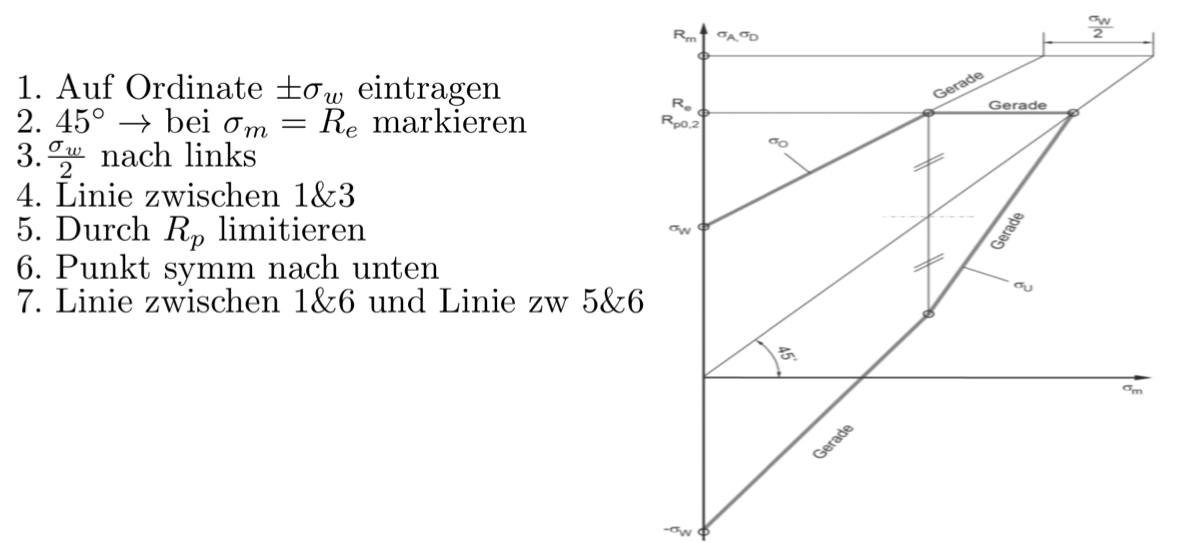
\includegraphics[width=\linewidth]{06/smith_diagramm.jpeg}
    
    